\documentclass[class=report, crop=false, 12pt,a4paper]{standalone}
\usepackage{enumitem}
\usepackage{multicol}
\usepackage{graphicx}
\usepackage{float}
\usepackage{amsmath}
\usepackage{amssymb}
\usepackage{mathtools}
\usepackage{siunitx}
\usepackage{commath}
\usepackage{array}
\usepackage{natbib}
\usepackage{tikz}
\usepackage{cancel}
\usepackage[a4paper,width=150mm,top=25mm,bottom=25mm]{geometry}
\allowdisplaybreaks
\setlength{\parindent}{0pt}
\numberwithin{equation}{section}
\begin{document}
\begin{center}
  09/03/2021
\end{center}
\section{Overview of Gas Turbine Systems}
Applications of Gas Turbines:
\begin{itemize}[noitemsep]
  \item Aircraft propulsion
  \item Marine propulsion
  \item Stationary power plants for electricity generation
\end{itemize}
\subsection{Schematic of a Gas Turbine Aeroengine}
\begin{figure}[H]
  \centering
  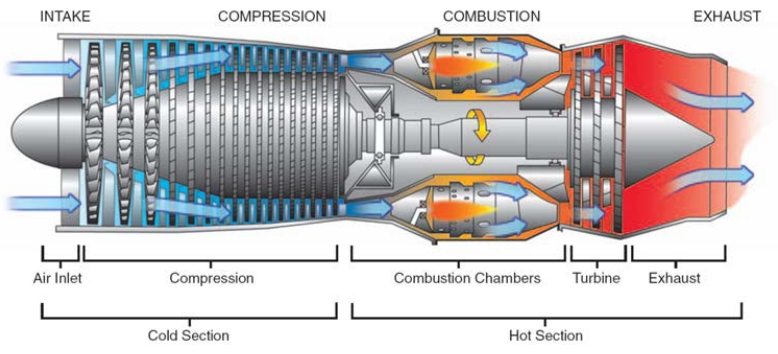
\includegraphics[width = 1 \textwidth]{../img/diagram151.png}
  \caption{}
\end{figure}
\section{Ideal Air-Standard Joule-Brayton Cycle}
Assumptions:
\begin{itemize}[noitemsep]
  \item The working fluid is air, which is assumed to be an ideal gas. 
  \item The temperature rise that would be brought about by combustion is accomplished by a heat transfer from an external source.
  \item Regard the turbine exhaust air as restored to the compressor inlet state by passing through a heat exchanger
\end{itemize}
\begin{figure}[H]
  \centering
  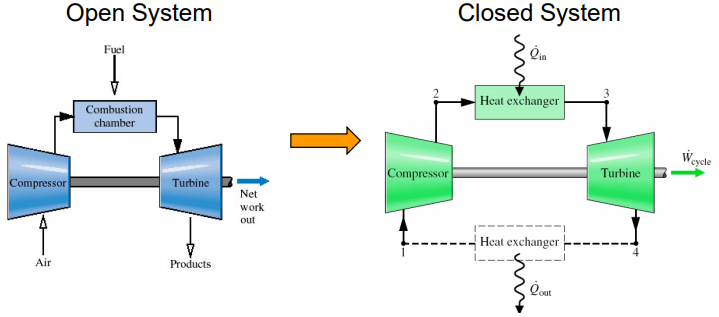
\includegraphics[width = 1 \textwidth]{../img/diagram152.png}
  \caption{}
\end{figure}
Ignoring irreversibilities in the various component:
\begin{itemize}[noitemsep]
  \item No frictional pressure drops through heat exchangers. 
  \item No heat transfers to the surroundings in heat exchangers.
  \item Isentropic expansion and compression in turbine and compressor.
\end{itemize}
\begin{figure}[H]
  \centering
  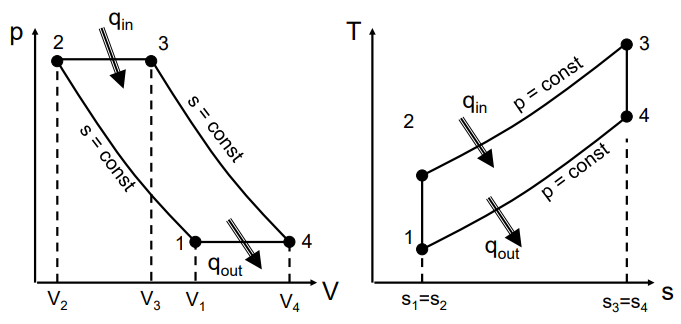
\includegraphics[width = 0.9 \textwidth]{../img/diagram153.png}
  \caption{}
\end{figure}
\subsection{Brayton Cycle}
Comparison with vapour power cycle:
\begin{itemize}[noitemsep]
  \item \textbf{High power output-to-weight ratio} $\longrightarrow$ lighter and more compact 
  \item \textbf{Lower pressure ratios}, higher volume based on gas vs. liquid compression (Liquid is difficult to be compressed)
  \item \textbf{Lower efficiencies} based on non-isothermal heat addition and heat rejection
\end{itemize}
Comparison with Otto and Diesel cycles:
\begin{itemize}
  \item $4\longrightarrow 1:$ constant pressure vs. constant volume process (both Otto and Diesel cycles)
  \item $2\longrightarrow 3:$ constant pressure vs. constant volume process (Otto cycle only)
\end{itemize}
In general, pressure rise much smaller for turbo-machinery than for reciprocating devices
\begin{figure}[H]
  \centering
  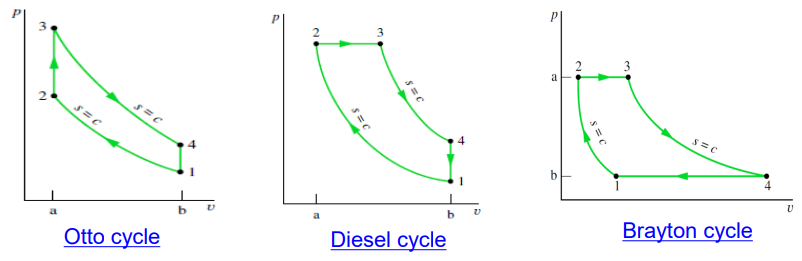
\includegraphics[width = 1 \textwidth]{../img/diagram154.png}
  \caption{}
\end{figure}
\subsection{First Law Analysis of Brayton Cycle}
\begin{figure}[H]
  \centering
  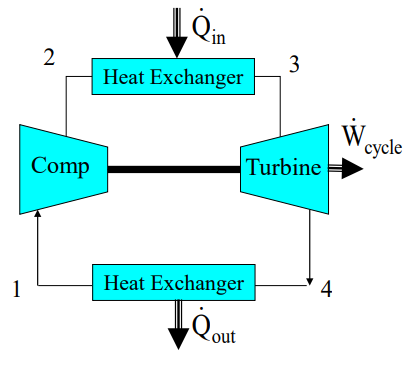
\includegraphics[width = 0.55 \textwidth]{../img/diagram155.png}
  \caption{}
\end{figure}
\subsubsection{1st Law, Energy Balance for Each Component:}
Work (Turbine and Compressor):
\begin{gather}
  \frac{\dot{W}_{T}}{\dot{m}} = h_3-h_4 \\[5pt]
  \frac{\dot{W}_{C}}{\dot{m}} = h_2-h_1
\end{gather}
Heat Transfer: 
\begin{gather}
  \frac{\dot{Q}_{in}}{\dot{m}} = h_3-h_2 \\[5pt]
  \frac{\dot{Q}_{out}}{\dot{m}} = h_4-h_1 
\end{gather}
Back Work Ratio:
\begin{gather}
  r_{BW} = \frac{\dot{W}_C}{\dot{W}_T} = \frac{h_2-h_1}{h_3-h_4}
\end{gather}
\begin{itemize}[noitemsep]
  \item For gas turbine, typically 40~80\%
  \item For vapour cycle, 1~2\%
\end{itemize}
\subsubsection{Thermal Efficiency:}
\begin{gather}
  \eta_{th} = \frac{w_{net}}{q_{in}} = \frac{w_T - w_C}{q_{in}} = \frac{q_{in} - |q_{out}|}{q_{in}} = 1 - \frac{|q_{out}|}{q_{in}}
\end{gather}
For closed cycle, SSSF (Steady-State, Steady-Flow), and $\Delta KE = \Delta PE = 0$
\begin{gather}
  \eta_{th} = 1-\frac{|q_{out}|}{q_{in}} = 1-\frac{h_4-h_1}{h_3-h_2}
\end{gather}
For constant specific heats (\textbf{cold air-standard analysis}):
\begin{gather}
  \eta_{th} = 1-\frac{c_p(T_4-T_1)}{c_p(T_3-T_2)} = 1-\frac{T_1}{T_2}\cdot\frac{\left(\frac{T_4}{T_1}-1\right)}{\left(\frac{T_3}{T_2}-1\right)}
  \label{Eff1}
\end{gather}
For an \textbf{isentropic process}:
\begin{gather}
  pv^k = \text{constant} \\[5pt]
  k = \frac{c_p}{c_v} \\[5pt]
  \text{Process}\ 1\longrightarrow 2: \ p_1v_1^k = p_2v_2^k \\[5pt]
  \longrightarrow \frac{v_1^k}{v_2^k} = \frac{p_2}{p_1} = \frac{\left(\frac{RT_1}{p_1}\right)^k}{\left(\frac{RT_2}{p_2}\right)^k} = \left(\frac{T_1}{T_2}\frac{p_2}{p_1}\right)^k \\[5pt]
  \longrightarrow \left(\frac{p_2}{p_1}\right)^{1/k} = \frac{T_1}{T_2}\frac{p_2}{p_1} \\[5pt]
  \longrightarrow \frac{T_2}{T_1} = \left(\frac{p_2}{p_1}\right)^{k/k}\cdot\left(\frac{p_2}{p_1}\right)^{-1/k} = \left(\frac{p_2}{p_1}\right)^{\frac{k-1}{k}} \\[5pt]
  \frac{T_4}{T_3} = \left(\frac{p_4}{p_3}\right)^{\frac{k-1}{k}} = \left(\frac{p_1}{p_2}\right)^{\frac{k-1}{k}} = \frac{T_1}{T_2} \\[5pt]
  \therefore \frac{T_4}{T_1} = \frac{T_3}{T_2}
\end{gather}
Therefore, going back to Equation (\ref{Eff1}): 
\begin{gather}
  \eta_{th} = 1-\frac{T_1}{T_2}\cdot\frac{\left(\frac{T_4}{T_1}-1\right)}{\left(\frac{T_3}{T_2}-1\right)} = 1-\frac{T_1}{T_2} \\[5pt]
  \frac{T_2}{T_1} = \left(\frac{p_2}{p_1}\right)^{\frac{k-1}{k}}
\end{gather}
Define temperature ratio:
\begin{gather}
  \tau = \frac{T_3}{T_1}
\end{gather}
Define pressure ratio: 
\begin{gather}
  r_p = \frac{p_2}{p_1} \\[5pt]
  \mathbf{\therefore \eta_{th} = 1-\frac{1}{r_p^{\frac{k-1}{k}}}}
\end{gather}
\subsection{Effects of Pressure Ratio on Ideal Cold Air-standard Brayton Cycle}
\begin{itemize}[noitemsep]
  \item If $r_p \uparrow$, then $\eta_{th} \uparrow$
  \item If $r_p$ is fixed, $q_{in}\uparrow$, then $w_{net}\uparrow$ but $\eta_{th}$ is not changed
\end{itemize}
\begin{figure}[H]
  \begin{center}
    \begin{minipage}[b]{0.46\textwidth}
      \centering
      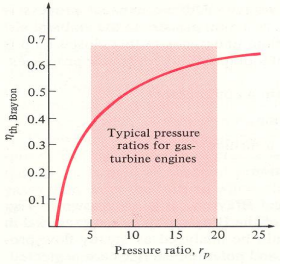
\includegraphics[width = 0.85 \textwidth]{../img/diagram156.png}
      \caption{}
    \end{minipage}
    \begin{minipage}[b]{0.46\textwidth}
      \centering
      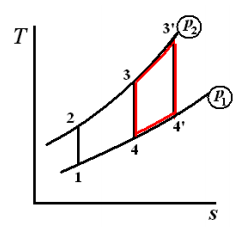
\includegraphics[width = 0.85 \textwidth]{../img/diagram157.png}
      \caption{}
    \end{minipage}
  \end{center}
\end{figure}
In practice, work output and efficiency are both important
\begin{figure}[H]
  \centering
  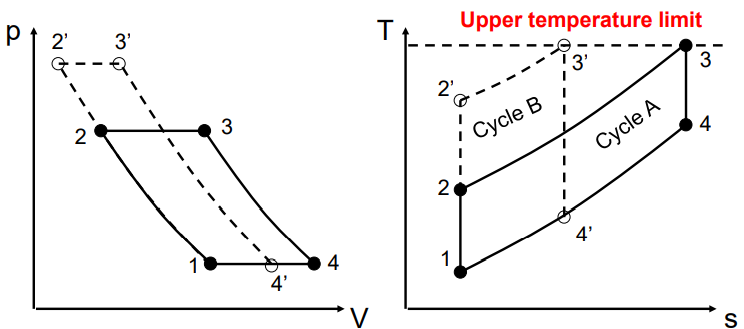
\includegraphics[width = 0.8 \textwidth]{../img/diagram158.png}
  \caption{}
\end{figure}
\subsection{Maximize Work Output with Fixed Temperature Ratio}
For given $T_1$ and $T_3$ (or temperature ratio), find:
\begin{itemize}[noitemsep]
  \item The optimal $T_2$, or
  \item The optimal pressure ratio $r_p$ that maximizes work output
\end{itemize}
\begin{figure}[H]
  \begin{center}
    \begin{minipage}[b]{0.46\textwidth}
      \centering
      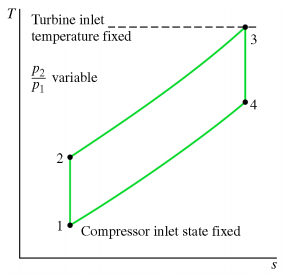
\includegraphics[width = 0.85 \textwidth]{../img/diagram159.png}
      \caption{}
    \end{minipage}
    \begin{minipage}[b]{0.46\textwidth}
      \centering
      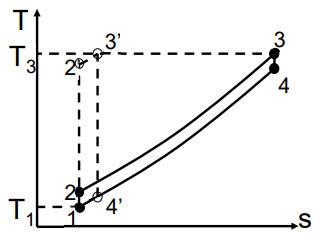
\includegraphics[width = 0.85 \textwidth]{../img/diagram160.png}
      \caption{}
    \end{minipage}
  \end{center}
\end{figure}
Limiting Cases:
\begin{enumerate}[noitemsep]
  \item $T_2 = T_3 \longrightarrow w_{net} = 0, \ \eta_{th} = \eta_{max}$
  \item $T_2 = T_1 \longrightarrow w_{net} = 0, \ \eta_{th} = 0$ 
\end{enumerate}
\subsubsection{Find Optimal $T_2$}
\begin{gather}
  w_{net} = w_T - |w_C| = q_{in} - |q_{out}|
\end{gather}
For constant specific heats:
\begin{gather}
  w_{net} = c_p(T_3-T_2) - c_p(T_4-T_1)
\end{gather}
For maximum $w_{net}$:
\begin{gather}
  \frac{dw_{net}}{dT_2} = 0 = c_p\left(\cancel{\frac{dT_3}{dT_2}}-1-\frac{dT_4}{dT_2}+\cancel{\frac{dT_1}{dT_2}}\right)
\end{gather}
Recalling:
\begin{gather}
  \frac{T_4}{T_1} = \frac{T_3}{T_2} \longrightarrow T_4 = \frac{T_1T_3}{T_2} \longrightarrow \frac{dT_4}{dT_2} = -\frac{T_1T_3}{T_2^2}
\end{gather}
Hence:
\begin{gather}
  \frac{w_{net}}{dT_2} = 0 = -1-\frac{dT_4}{dT_2} = -1+\frac{T_1T_3}{T_2^2} \\[5pt]
  \therefore T_2 = \sqrt{T_1T_3}
\end{gather}
\subsubsection{Find Optimal $r_p$}
\begin{gather}
  w_{net} = q_{in} - q_{out} = cp\left[(T_3-T_2) - (T_4-T_1)\right] \\[5pt]
  = c_p T_1\left[\left(\frac{T_3}{T_1}-\frac{T_2}{T_1}\right)-\left(\frac{T_4}{T_1}-1\right)\right] \\[5pt]
  = c_p T_1\left[\left(\frac{T_3}{T_1}-\frac{T_2}{T_1}\right)-\left(\frac{T_3}{T_2}-1\right)\right] \\[5pt]
  = c_p T_1\left[\left(\frac{T_3}{T_1}-\frac{T_2}{T_1}\right)-\left(\frac{T_3}{T_1}\frac{T_1}{T_2}-1\right)\right] \\[5pt]
  \tau = \frac{T_3}{T_1} \\[5pt]
  = c_p T_1\left[\tau - r_p^{\frac{k-1}{k}} - \left(\tau r_p^{-\frac{k-1}{k}}-1\right)\right]
\end{gather}
Let:
\begin{gather}
  \frac{\partial w_{net}}{dr_p} = 0
\end{gather}
Hence:
\begin{gather}
  r_p = \tau^{\frac{k}{2(k-1)}} \implies w_{net} \rightarrow w_{net,max} \\[5pt]
  w_{net} = c_p T_1 \left(r_p^{\frac{k-1}{k}}-1\right)\left(\frac{\tau}{r_p^{\frac{k-1}{k}}}-1\right)
\end{gather}
For each temperature ratio, there is an optimum pressure ratio to achieve the maximum work output. \\\\
The larger the temperature ratio, the larger the optimum pressure ratio, i.e., the larger the thermal efficiency when the maximum output is acquired. \\\\
\textbf{$T_3$ is a key parameter in practice}
\begin{figure}[H]
  \centering
  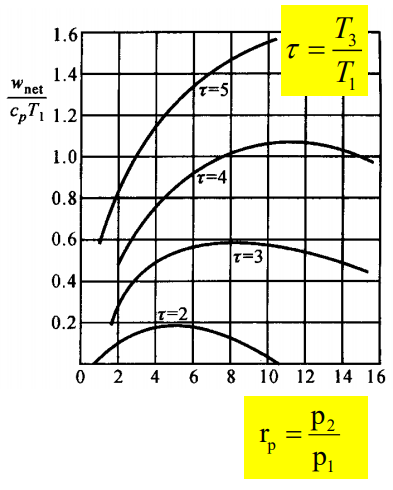
\includegraphics[width = 0.4 \textwidth]{../img/diagram161.png}
  \caption{}
\end{figure}
\section{Brayton Cycles with Irreversibilities}
\begin{figure}[H]
  \begin{center}
    \begin{minipage}[b]{0.46\textwidth}
      \centering
      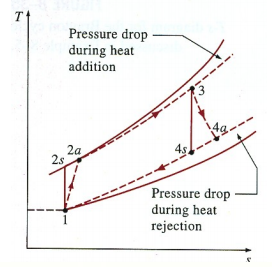
\includegraphics[width = 0.85 \textwidth]{../img/diagram162.png}
      \caption{}
    \end{minipage}
    \begin{minipage}[b]{0.46\textwidth}
      \centering
      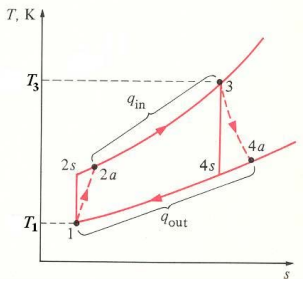
\includegraphics[width = 0.85 \textwidth]{../img/diagram163.png}
      \caption{}
    \end{minipage}
  \end{center}
\end{figure}
Deviation of actual gas-turbine cycles from idealized ones:
\begin{gather}
  \eta_C = \frac{w_s}{w_a} = \frac{h_{2s}-h_1}{h_{2a}-h_1} \\[5pt]
  \eta_T = \frac{w_a}{w_s} = \frac{h_3-h_{4a}}{h_3-h_{4s}}
\end{gather}
Note:
\begin{itemize}[noitemsep]
  \item $T_2 > T_{2s}$ if $p_2 = p_{2s}$
  \item $T_4 > T_{4s}$ if $p_4 = p_{4s}$
\end{itemize}
Irreversibilities convert mechanical energy to thermal loss through friction.
\subsubsection{1st Law, Energy Balance for Each Component:}
\begin{figure}[H]
  \centering
  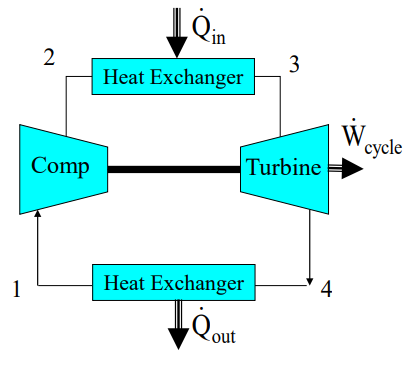
\includegraphics[width = 0.55 \textwidth]{../img/diagram155.png}
  \caption{}
\end{figure}
Work (Turbine and Compressor):
\begin{gather}
  \frac{\dot{W}_T}{\dot{m}} = h_3-h_{4a} \\[5pt]
  \frac{\dot{W}_C}{\dot{m}} = h_{2a}-h_1
\end{gather}
Heat Transfer:
\begin{gather}
  \frac{\dot{Q}_{in}}{\dot{m}} = h_3-h_{2a} \\[5pt]
  \frac{\dot{Q}_{out}}{\dot{m}} = h_{4a}-h_1
\end{gather}
Back Work Ratio:
\begin{gather}
  r_{BW} = \frac{\dot{W}_C}{\dot{W}_T} = \frac{h_{2a}-h_1}{h_3-h_{4a}}
\end{gather}
Compressor Efficiency and Work:
\begin{gather}
  \eta_C = \frac{w_{CS}}{w'_C} = \frac{h_{2s}-h_1}{h_{2a}-h_1} \\[5pt]
  w'_C = \frac{h_{2s}-h_1}{\eta_C} \\[5pt]
  h_{2a} = h_1 + \frac{h_{2s}-h_1}{\eta_C}
\end{gather}
Turbine Efficiency and Work:
\begin{gather}
  \eta_T = \frac{w'_{t,T}}{w_{t,T}} = \frac{h_3-h_{4a}}{h_3-h_{4s}} \\[5pt]
  w'_{t,T} = \eta_T(h_3-h_{4s}) \\[5pt]
  h_{4a} = h_3-\eta_T(h_3-h_{4s})
\end{gather}
Actual Efficiency, Work and Heat Transfer with Irreversibilities:
\begin{gather}
  \eta_i = \frac{w'_{net}}{q'_{in}} \\[5pt]
  w'_{net} = w'_{t,T} - w'_C = \eta_T(h_3-h_{4s})-\frac{h_{2s}-h_1}{\eta_C} \\[5pt]
  q'_{in} = h_3-h_2 = h_3-h_1-\frac{h_{2s}-h_1}{\eta_C} \\[5pt]
  \eta_i = \frac{\eta_T(h_3-h_{4s})-\frac{h_{2s}-h_1}{\eta_C}}{h_3-h_1-\frac{h_{2s}-h_1}{\eta_C}}
\end{gather}
\subsubsection{Example:}
\begin{figure}[H]
  \centering
  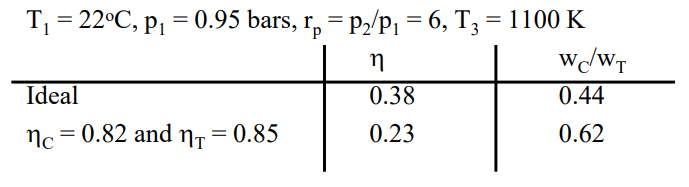
\includegraphics[width = 0.8 \textwidth]{../img/diagram164.png}
  \caption{}
\end{figure}
Notes:
\begin{itemize}[noitemsep]
  \item The overall efficiency is reduced by 40\%
  \item Gas turbine performance is very sensitive to turbine and compressor efficiencies, because the overall efficiency is low.
\end{itemize}
\section{Regenerative Brayton Cycle}
Introduce “regeneration” to boost overall efficiency: 
\begin{itemize}[noitemsep]
  \item Idea: reclaim “waste” heat in the exhaust normally lost to the ambient.
\end{itemize}
Regenerative open Brayton cycle:
\begin{figure}[H]
  \centering
  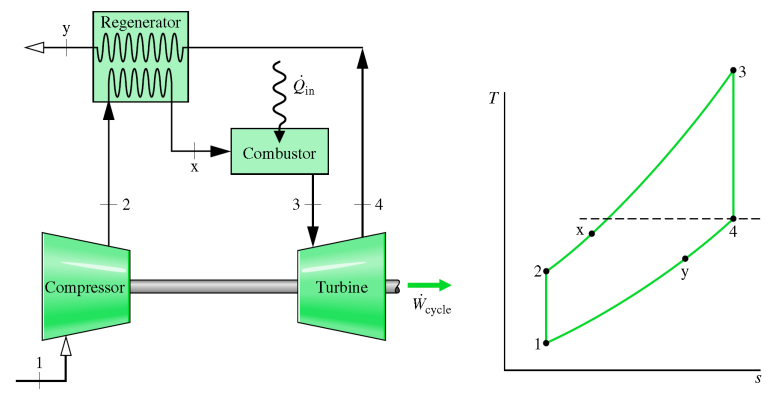
\includegraphics[width = 0.95 \textwidth]{../img/diagram165.png}
  \caption{}
\end{figure}
\begin{figure}[H]
  \centering
  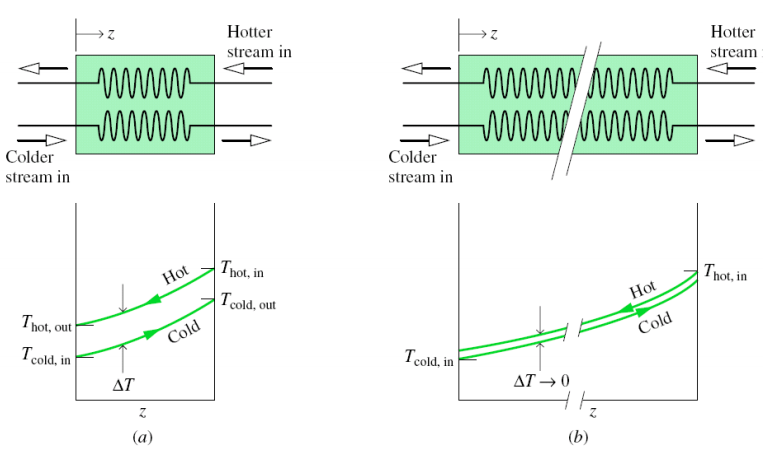
\includegraphics[width = 0.95 \textwidth]{../img/diagram166.png}
  \caption{Temperature distributions in counterflow heat exchangers (a) Actual | (b) Reversible}
\end{figure}
\subsection{Regenerator Effectiveness}
Regenerator Effectiveness is defined as:
\begin{gather}
  \eta_{reg} = \frac{h_x-h_2}{h_4-h_2} \\[5pt]
  \eta_{reg} = 60 \approx 80\% \ \text{typically}
\end{gather}
\subsection{Thermal Efficiency of Ideal Regenerative Brayton Cycle}
Work and heat analysis:
\begin{gather}
  \frac{\dot{W}_T}{\dot{m}} = h_3-h_4 \\[5pt]
  \frac{\dot{W}_C}{\dot{m}} = h_2-h_1 \\[5pt]
  \frac{\dot{Q}_{in}}{\dot{m}} = h_3-h_x
\end{gather}
Thermal efficiency: 
\begin{gather}
  \eta = \frac{\frac{\dot{W}_T}{\dot{m}}-\frac{\dot{W}_C}{\dot{m}}}{\frac{\dot{Q}_{in}}{\dot{m}}} = \frac{(h_3-h_4)-(h_2-h_1)}{h_3-h_x}
\end{gather}
Regenerator Effectiveness:
\begin{gather}
  \eta_{reg} = \frac{h_x-h_2}{h_4-h_2} \\[5pt]
  h_x = \eta_{reg}(h_4-h_2)+h_2
\end{gather}
Finally, ideal thermal efficiency:
\begin{gather}
  \eta = \frac{(h_3-h_4)-(h_2-h_1)}{h_3-h_x} = \frac{(h_3-h_4)-(h_2-h_1)}{h_3-\eta_{reg}(h_4-h_2)-h_2}
\end{gather}
\subsection{Thermal Efficiency of Non-ideal Regenerative Brayton Cycle}
\begin{figure}[H]
  \begin{center}
    \begin{minipage}[b]{0.42\textwidth}
      \centering
      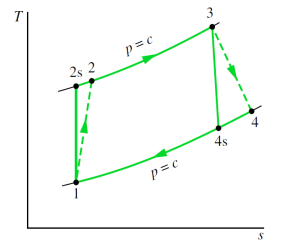
\includegraphics[width = 0.85 \textwidth]{../img/diagram167.png}
      \caption{}
    \end{minipage}
    \begin{minipage}[b]{0.42\textwidth}
      \centering
      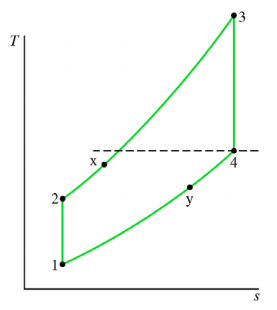
\includegraphics[width = 0.85 \textwidth]{../img/diagram168.png}
      \caption{}
    \end{minipage}
  \end{center}
\end{figure}
Efficiency of turbine:
\begin{gather}
  \eta_T = \frac{h_3-h_4}{h_3-h_{4s}} \\[5pt]
  h_4 = h_4-\eta_T(h_3-h_{4s})
\end{gather}
Efficiency of compressor:
\begin{gather}
  \eta_C = \frac{h_{2s}-h_1}{h_2-h_1} \\[5pt]
  h_2 = h_1 + \frac{h_{2s}-h_1}{\eta_C}
\end{gather}
Finally, non-ideal thermal efficiency: 
\begin{gather}
  \eta = \frac{(h_3-h_4)-(h_2-h_1)}{h_3-h_x} = \frac{(h_3-h_4)-(h_2-h_1)}{h_3-\eta_{reg}(h_4-h_2)-h_2} \\[5pt]
  \eta = \frac{\eta_T(h_3-h_{4s})-\frac{h_{2s}-h_1}{\eta_C}}{h_3-\eta_{reg}\left[h_3-\eta_T(h_3-h_{4s})-h_1-\frac{h_{2s}-h_1}{\eta_C}\right]\frac{h_{2s}-h_1}{\eta_C}  }
\end{gather}
\section{Gas Turbines with Reheat and Intercooling}
\subsection{Gas Turbines with Reheat}
\begin{itemize}[noitemsep]
  \item Two-stage gas turbine with reheat in between
  \item The net work per cycle is increased with reheat than without
  \item The thermal efficiency may or may not increase due to reheat
  \item Gas turbine with reheat has greater potential for regeneration
\end{itemize}
\begin{figure}[H]
  \centering
  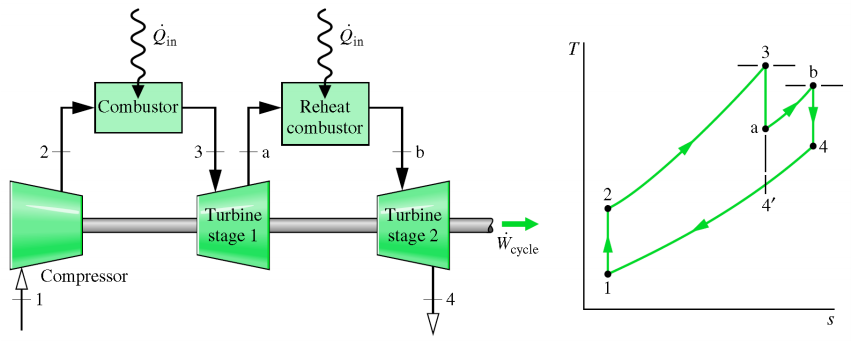
\includegraphics[width = 1 \textwidth]{../img/diagram169.png}
  \caption{}
\end{figure}
\subsection{Compression with Intercooling}
\begin{itemize}[noitemsep]
  \item Compression work is significant in gas turbines
  \item Adiabatic compression requires more work than compression with cooling
  \item Cooling during compression is hard to achieve due to heat transfer rate limit
  \item Intercooling between compression stages is more efficient
\end{itemize}
\begin{figure}[H]
  \centering
  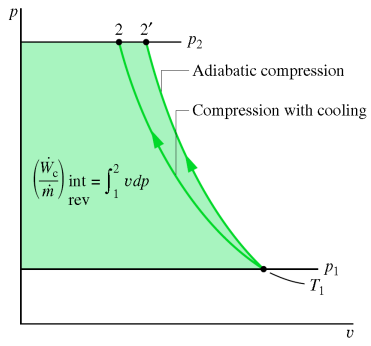
\includegraphics[width = 0.45 \textwidth]{../img/diagram170.png}
  \caption{Internally reversible compression between two fixed pressures}
\end{figure}
\subsection{Two-stage Compressor with Intercooler}
\begin{itemize}[noitemsep]
  \item Process 1-c and d-2: isentropic compression
  \item Process c-d: constant-pressure cooling
  \item The net work of gas turbine is increased due to decreased compression work
  \item Cycle efficiency is not necessarily increased due to lower temperature at combustor inlet
  \item Potential for regeneration is increased
\end{itemize}
\begin{figure}[H]
  \centering
  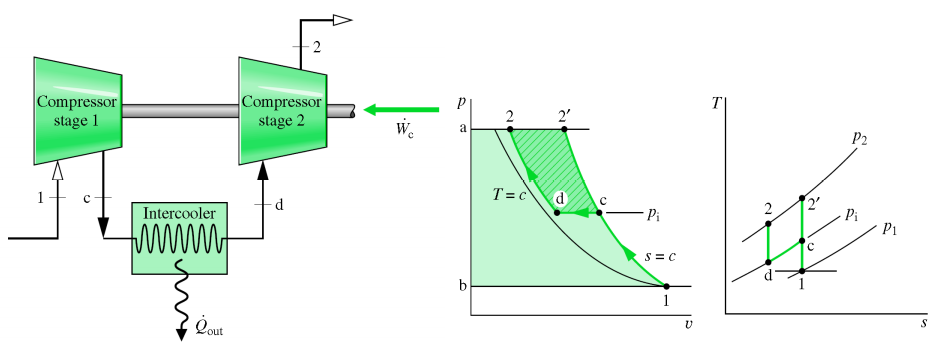
\includegraphics[width = 1 \textwidth]{../img/diagram171.png}
  \caption{}
\end{figure}
\subsection{Regenerative GT with Reheat \& Intercooling}
\begin{figure}[H]
  \centering
  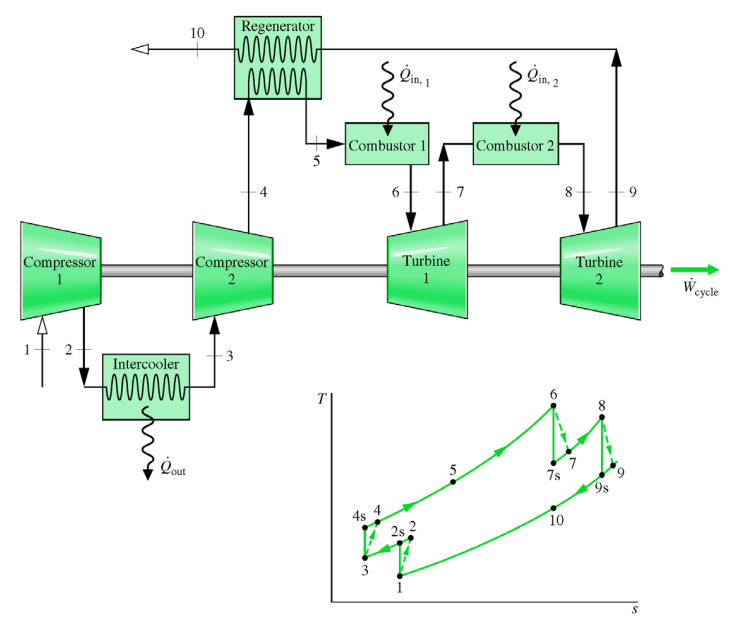
\includegraphics[width = 1 \textwidth]{../img/diagram172.png}
  \caption{}
\end{figure}
\section{Gas Turbine – Steam Turbine Combined Cycle}
The combustion of fossil fuel can produce much higher temperature than that of evaporation temperature of the steam (due to the limitation of critical temperature of the water), potentially producing large exergy destruction during heat transfer process in boiler(~30\%). \\\\
The gas turbine can operate at higher temperature, reducing exergy destruction due to heat transfer. \\\\
The exhaust gas temperature after expansion in gas turbine is high enough to transfer heat to the water to generate steam for the vapour power cycle. \\\\
By combining gas turbine plant cycle with steam power plant cycle, the use of thermal energy is more efficient. 
\begin{figure}[H]
  \centering
  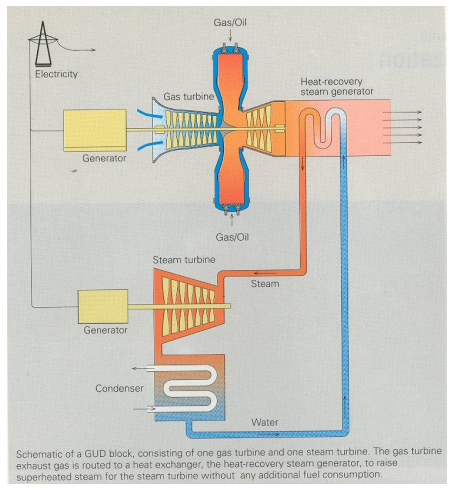
\includegraphics[width = 0.7 \textwidth]{../img/diagram173.png}
  \caption{}
\end{figure}
The energy balance in heat recovery steam generator: 
\begin{gather}
  \dot{m}_v(h_7-h_6) = \dot{m}_g(h_4-h_5)
\end{gather}
\begin{figure}[H]
  \centering
  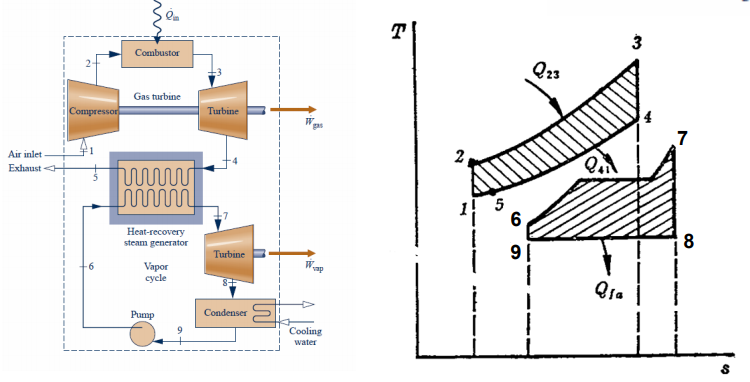
\includegraphics[width = 1 \textwidth]{../img/diagram174.png}
  \caption{}
\end{figure}
The overall thermal efficiency:
\begin{gather}
  \eta_t = 1-\frac{\dot{Q}_{out}}{\dot{Q}_{in}} = 1-\frac{\dot{m}_g(h_5-h_1)+\dot{m}_v(h_8-h_9)}{\dot{m}_g(h_3-h_2)}
\end{gather}
\subsection{Gas Turbine – Steam Turbine Combined Power Cycle with Cogeneration}
Generate both electricity and heat to cater for the demand of electricity, steam for industry, and steam for domestic heating purpose at the same time. \\\\
Higher overall “energy” utilization efficiency, because less heat is rejected to the environment. \\\\
If steam for industry and for domestic heating be generated through independent boiler, a large amount of “exergy” will be wasted. 
\section{Summary}
\begin{itemize}[noitemsep]
  \item Thermal efficiency of ideal air-standard Jouel- Brayton Cycle is dependent on pressure ratio of the compressor
  \item Regeneration in gas turbines increases thermal efficiency
  \item Reheat and compression intercooling increase work output
  \item Gas turbine and steam turbine combined cycle has high overall energy efficienc
\end{itemize}
\end{document}